\begin{figure*}
  \begin{center}
    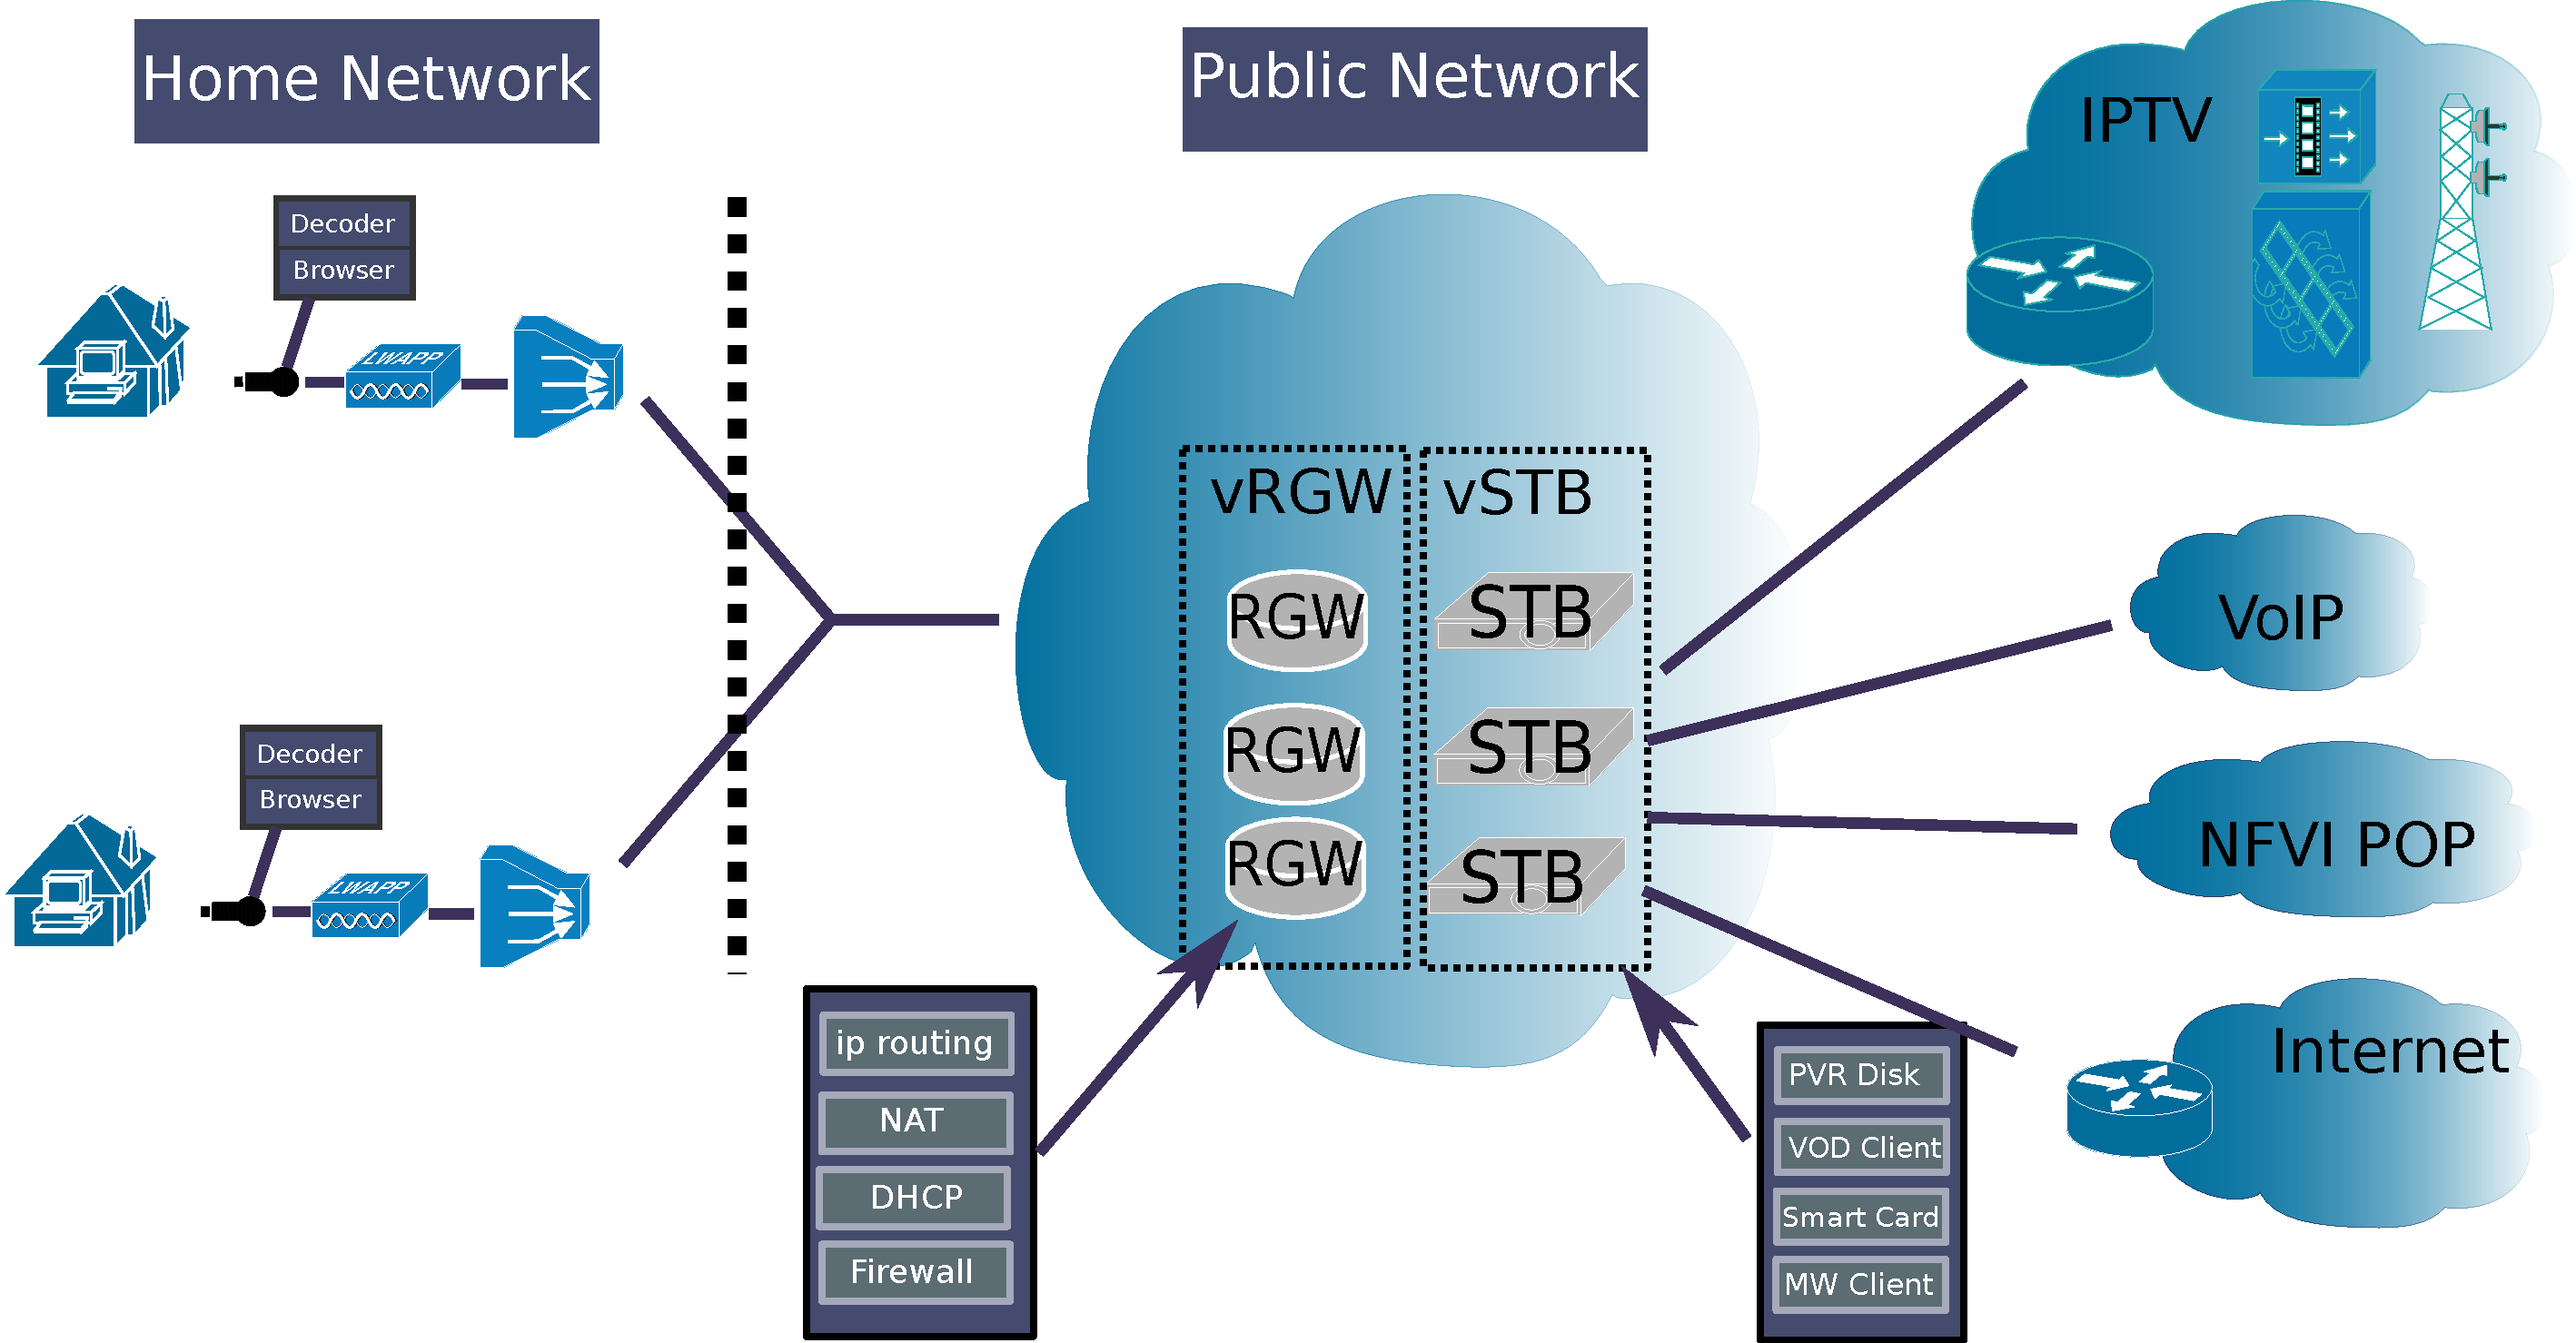
\includegraphics[width=0.75\textwidth]{fig/etsi-virtualisation-home-env.pdf}
  \end{center}
  \caption{ Virtualisation of the home environment according to ETSI.
    \label{fig:etsi-vision}
  }
\end{figure*}

Since the introduction of high speed Internet technologies such as xDSL and FTTx, End-Users' demands for Internet services grow at an exponential rate.
According to Akamai, the most popular Content Delivery Network (CDN) provider, the average bandwidth has continued to globally increase by 65\% in the second quarter of 2014 \cite{_akamais_2014} compared to 2013. 
Moreover, it is expected that IP video traffic will reach almost 80\% of all consumer Internet traffic in 2018 \footnote{CISCO forecast white paper http://bit.ly/LVhmuL }. To cope with this drastic evolution, new concepts emerge, such as Network Function Virtualisation (NFV), and they appear to be very promising especially for the delivery aspects of video content.

The Home Gateways (HG), for the networking part, and the Set-Top-Boxes (STB), for the rendering part, constitute two of the major equipments in charge of processing media content and delivering it to a number of devices such as screens, smartphones, tablets, computers, mobile devices and security appliances.
HG and STB are placed on the last portion of the Service Provider's (SP) network under the conjoined responsibility of the End-User and the SP.
HG \& STB usually consist of self-contained components, using internally stored firmware.
When new configuration updates are released, new model and firmware upgrades are being constantly pushed to the market.
The hardware and software fragmentation becomes more and more prominent, increasing operational expenses (OPEX). 

In the highly competitive industry of Service Providers, where the arrival of a new player can be a game changer, new services and new norms are frequently rolled out.	
The impact on Customer Premise Equipment (CPE), like HG or STB, can be huge, as software updates can be insufficient to cover new requirements.
Updating hardware is vital, however this leads to high capital expenditure (CAPEX).
For instance, most STBs cannot decode the new video format standard  High Efficiency Video Coding (HEVC). 
The challenge for SP is threefold: they must find a way to tackle with disruptive changes brought by End-User new expectations (like adopting 4K or 8K TV) and roll out new services to find new revenue streams while lowering expenses induced by replacing their network hardware devices.

Cloud Computing promotes the deployment of IT services on commodity servers has not reached the telco world so far, due to its lack of standardization and doubts regarding its ability to deliver telecom services. 
Drawing on this observation, the European Telecommunications Standards Institute (ETSI) issued a seminal white paper \cite{_network_2012}, introducing the notion of Network Function Virtualisation (NFV) and launched an Industry Specification Group for NFV, producing frequent white papers and design documents.
The whole NFV concept aims at creating a reference architecture and a standardized approach to achieve carrier grade virtualisation of existing network functions currently performed by hardware middle boxes, on commodity servers.
Network equipment vitalization touches a broad range of devices, including HG and STB as ETSI mentions in the “Virtualisation of the Home Environment” section of \cite{_network_2013}. 

As interest in NFV grows, several field studies are performed to verify it can be launched to market.
However, the transition from the current monolithic firmware based CPE to a proper full cloud solution is unlikely to happen immediately. Telefonica, the precusor in this domain mentionned in \cite{enrique_blanco_telefonica_2015} that the first commercial deployments of vCPE will occur during in 2015.

In this paper, we will study the feasibility of a NFV based HG.  To this end, we introduce a novel  approach centred around the concept of Surrogate VNF deployed on the Home Gateway.
It will serve as a drop-in replacement for an existing function by leveraging the usage of Open Services Gateway initiative (OSGi\footnote{http://www.osgi.org/}) technology promoted by the Home Gateway Initiative.
The rest of this paper is organized as follows.
~Section \ref{sec:background}, explores the related work on the current and next generation Home Gateway architectures and reviews existing approaches for virtualising CPEs in general.
Section \ref{sec:migrating} presents the overall concept of our SvNF-based solution. Section \ref{sec:results} is dedicated to its evaluation through experimentations and simulations. Finally, section \ref{sec:conclusion} concludes and outlines further possible work.


